\chapter{深度优先搜索}


\section{Palindrome Partitioning} %%%%%%%%%%%%%%%%%%%%%%%%%%%%%%
\label{sec:palindrome-partitioning}


\subsubsection{描述}
Given a string s, partition s such that every substring of the partition is a palindrome.

Return all possible palindrome partitioning of s.

For example, given \code{s = "aab"},
Return
\begin{Code}
  [
    ["aa","b"],
    ["a","a","b"]
  ]
\end{Code}


\subsubsection{分析}
在每一步都可以判断中间结果是否为合法结果,用回溯法。

一个长度为n的字符串,有$n-1$个地方可以砍断,每个地方可断可不断,因此复杂度为$O(2^{n-1})$


\subsubsection{深搜1}
\begin{Code}
//LeetCode, Palindrome Partitioning
// 时间复杂度O(2^n),空间复杂度O(n)
class Solution {
public:
    vector<vector<string>> partition(string s) {
        vector<vector<string>> result;
        vector<string> path;  // 一个partition方案
        dfs(s, path, result, 0, 1);
        return result;
    }

    // s[0, prev-1]之间已经处理,保证是回文串
    // prev 表示s[prev-1]与s[prev]之间的空隙位置,start同理
    void dfs(string &s, vector<string>& path,
            vector<vector<string>> &result, size_t prev, size_t start) {
        if (start == s.size()) { // 最后一个隔板
            if (isPalindrome(s, prev, start - 1)) { // 必须使用
                path.push_back(s.substr(prev, start - prev));
                result.push_back(path);
                path.pop_back();
            }
            return;
        }
        // 不断开
        dfs(s, path, result, prev, start + 1);
        // 如果[prev, start-1] 是回文,则可以断开,也可以不断开(上一行已经做了)
        if (isPalindrome(s, prev, start - 1)) {
            // 断开
            path.push_back(s.substr(prev, start - prev));
            dfs(s, path, result, start, start + 1);
            path.pop_back();
        }
    }

    bool isPalindrome(const string &s, int start, int end) {
        while (s[start] == s[end]) {
            ++start;
            --end;
        }
        return start >= end;
    }
};
\end{Code}

\subsubsection{深搜2}
另一种写法,更加简洁。这种写法也在 Combination Sum, Combination Sum II 中出现过。
\begin{Code}
//LeetCode, Palindrome Partitioning
// 时间复杂度O(2^n),空间复杂度O(n)
class Solution {
public:
    vector<vector<string>> partition(string s) {
        vector<vector<string>> result;
        vector<string> path;  // 一个partition方案
        DFS(s, path, result, 0);
        return result;
    }
    // 搜索必须以s[start]开头的partition方案
    void DFS(string &s, vector<string>& path,
            vector<vector<string>> &result, int start) {
        if (start == s.size()) {
            result.push_back(path);
            return;
        }
        for (int i = start; i < s.size(); i++) {
            if (isPalindrome(s, start, i)) { // 从i位置砍一刀
                path.push_back(s.substr(start, i - start + 1));
                DFS(s, path, result, i + 1);  // 继续往下砍
                path.pop_back(); // 撤销上上行
            }
        }
    }
    bool isPalindrome(const string &s, int start, int end) {
        while (s[start] == s[end]) {
            ++start;
            --end;
        }
        return start >= end;
    }
};
\end{Code}


\subsubsection{动规}
\begin{Code}
// LeetCode, Palindrome Partitioning
// 动规,时间复杂度O(n^2),空间复杂度O(1)
class Solution {
public:
    vector<vector<string> > partition(string s) {
        const int n = s.size();
        bool p[n][n]; // whether s[i,j] is palindrome
        fill_n(&p[0][0], n * n, false);
        for (int i = n - 1; i >= 0; --i)
            for (int j = i; j < n; ++j)
                p[i][j] = s[i] == s[j] && ((j - i < 2) || p[i + 1][j - 1]);

        vector<vector<string> > sub_palins[n]; // sub palindromes of s[0,i]
        for (int i = n - 1; i >= 0; --i) {
            for (int j = i; j < n; ++j)
                if (p[i][j]) {
                    const string palindrome = s.substr(i, j - i + 1);
                    if (j + 1 < n) {
                        for (auto v : sub_palins[j + 1]) {
                            v.insert(v.begin(), palindrome);
                            sub_palins[i].push_back(v);
                        }
                    } else {
                        sub_palins[i].push_back(vector<string> { palindrome });
                    }
                }
        }
        return sub_palins[0];
    }
};
\end{Code}


\subsubsection{相关题目}

\begindot
\item Palindrome Partitioning II,见 \S \ref{sec:palindrome-partitioning-ii}
\myenddot


\section{Unique Paths} %%%%%%%%%%%%%%%%%%%%%%%%%%%%%%
\label{sec:unique-paths}


\subsubsection{描述}
A robot is located at the top-left corner of a $m \times n$ grid (marked 'Start' in the diagram below).

The robot can only move either down or right at any point in time. The robot is trying to reach the bottom-right corner of the grid (marked 'Finish' in the diagram below).

How many possible unique paths are there?

\begin{center}
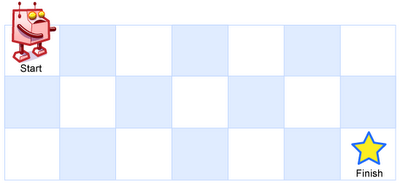
\includegraphics[width=200pt]{robot-maze.png}\\
\figcaption{Above is a $3 \times 7$ grid. How many possible unique paths are there?}\label{fig:unique-paths}
\end{center}

\textbf{Note}: $m$ and $n$ will be at most 100.


\subsection{深搜}
深搜,小集合可以过,大集合会超时

\subsubsection{代码}
\begin{Code}
// LeetCode, Unique Paths
// 深搜,小集合可以过,大集合会超时
// 时间复杂度O(n^4),空间复杂度O(n)
class Solution {
public:
    int uniquePaths(int m, int n) {
        if (m < 1 || n < 1) return 0; // 终止条件

        if (m == 1 && n == 1) return 1; // 收敛条件

        return uniquePaths(m - 1, n) + uniquePaths(m, n - 1);
    }
};
\end{Code}


\subsection{备忘录法}
给前面的深搜,加个缓存,就可以过大集合了。即备忘录法。

\subsubsection{代码}
\begin{Code}
// LeetCode, Unique Paths
// 深搜 + 缓存,即备忘录法
// 时间复杂度O(n^2),空间复杂度O(n^2)
class Solution {
public:
    int uniquePaths(int m, int n) {
        // 0行和0列未使用
        this->f = vector<vector<int> >(m + 1, vector<int>(n + 1, 0));
        return dfs(m, n);
    }
private:
    vector<vector<int> > f;  // 缓存

    int dfs(int x, int y) {
        if (x < 1 || y < 1) return 0; // 数据非法,终止条件

        if (x == 1 && y == 1) return 1; // 回到起点,收敛条件

        return getOrUpdate(x - 1, y) + getOrUpdate(x, y - 1);
    }

    int getOrUpdate(int x, int y) {
        if (f[x][y] > 0) return f[x][y];
        else return f[x][y] = dfs(x, y);
    }
};
\end{Code}


\subsection{动规}
既然可以用备忘录法自顶向下解决,也一定可以用动规自底向上解决。

设状态为\fn{f[i][j]},表示从起点$(1,1)$到达$(i,j)$的路线条数,则状态转移方程为:
\begin{Code}
f[i][j]=f[i-1][j]+f[i][j-1]
\end{Code}


\subsubsection{代码}
\begin{Code}
// LeetCode, Unique Paths
// 动规,滚动数组
// 时间复杂度O(n^2),空间复杂度O(n)
class Solution {
public:
    int uniquePaths(int m, int n) {
        vector<int> f(n, 0);
        f[0] = 1;
        for (int i = 0; i < m; i++) {
            for (int j = 1; j < n; j++) {
                // 左边的f[j],表示更新后的f[j],与公式中的f[i[[j]对应
                // 右边的f[j],表示老的f[j],与公式中的f[i-1][j]对应
                f[j] = f[j - 1] + f[j];
            }
        }
        return f[n - 1];
    }
};
\end{Code}


\subsection{数学公式}
一个$m$行,$n$列的矩阵,机器人从左上走到右下总共需要的步数是$m+n-2$,其中向下走的步数是$m-1$,因此问题变成了在$m+n-2$个操作中,选择$m–1$个时间点向下走,选择方式有多少种。即 $C_{m+n-2}^{m-1}$ 。

\subsubsection{代码}
\begin{Code}
// LeetCode, Unique Paths
// 数学公式
class Solution {
public:
    typedef long long int64_t;
    // 求阶乘, n!/(start-1)!,即 n*(n-1)...start,要求 n >= 1
    static int64_t factor(int n, int start = 1) {
        int64_t  ret = 1;
        for(int i = start; i <= n; ++i)
            ret *= i;
        return ret;
    }
    // 求组合数 C_n^k
    static int64_t combination(int n, int k) {
        // 常数优化
        if (k == 0) return 1;
        if (k == 1) return n;

        int64_t ret = factor(n, k+1);
        ret /= factor(n - k);
        return ret;
    }

    int uniquePaths(int m, int n) {
        // max 可以防止n和k差距过大,从而防止combination()溢出
        return combination(m+n-2, max(m-1, n-1));
    }
};
\end{Code}


\subsubsection{相关题目}
\begindot
\item Unique Paths II,见 \S \ref{sec:unique-paths-ii}
\item Minimum Path Sum, 见 \S \ref{sec:minimum-path-sum}
\myenddot


\section{Unique Paths II} %%%%%%%%%%%%%%%%%%%%%%%%%%%%%%
\label{sec:unique-paths-ii}


\subsubsection{描述}
Follow up for "Unique Paths":

Now consider if some obstacles are added to the grids. How many unique paths would there be?

An obstacle and empty space is marked as 1 and 0 respectively in the grid.

For example,

There is one obstacle in the middle of a $3 \times 3$ grid as illustrated below.
\begin{Code}
[
  [0,0,0],
  [0,1,0],
  [0,0,0]
]
\end{Code}

The total number of unique paths is 2.

Note: $m$ and $n$ will be at most 100.


\subsection{备忘录法}
在上一题的基础上改一下即可。相比动规,简单得多。

\subsubsection{代码}
\begin{Code}
// LeetCode, Unique Paths II
// 深搜 + 缓存,即备忘录法
class Solution {
public:
    int uniquePathsWithObstacles(vector<vector<int> > &obstacleGrid) {
        const int m = obstacleGrid.size();
        const int n = obstacleGrid[0].size();
        // 0行和0列未使用
        this->f = vector<vector<int> >(m + 1, vector<int>(n + 1, 0));
        return dfs(obstacleGrid, m, n);
    }
private:
    vector<vector<int> > f;  // 缓存

    int dfs(const vector<vector<int> > &obstacleGrid,
            int x, int y) {
        if (x < 1 || y < 1) return 0; // 数据非法,终止条件

        // (x,y)是障碍
        if (obstacleGrid[x-1][y-1]) return 0;

        if (x == 1 and y == 1) return 1; // 回到起点,收敛条件

        return getOrUpdate(obstacleGrid, x - 1, y) +
                getOrUpdate(obstacleGrid, x, y - 1);
    }

    int getOrUpdate(const vector<vector<int> > &obstacleGrid,
            int x, int y) {
        if (f[x][y] > 0) return f[x][y];
        else return f[x][y] = dfs(obstacleGrid, x, y);
    }
};
\end{Code}


\subsection{动规}
与上一题类似,但要特别注意第一列的障碍。在上一题中,第一列全部是1,但是在这一题中不同,第一列如果某一行有障碍物,那么后面的行应该为0。


\subsubsection{代码}
\begin{Code}
// LeetCode, Unique Paths II
// 动规,滚动数组
// 时间复杂度O(n^2),空间复杂度O(n)
class Solution {
public:
    int uniquePathsWithObstacles(vector<vector<int> > &obstacleGrid) {
        const int m = obstacleGrid.size();
        const int n = obstacleGrid[0].size();
        if (obstacleGrid[0][0] || obstacleGrid[m-1][n-1]) return 0;

        vector<int> f(n, 0);
        f[0] = obstacleGrid[0][0] ? 0 : 1;

        for (int i = 0; i < m; i++)
            for (int j = 0; j < n; j++)
                f[j] = obstacleGrid[i][j] ? 0 : (j == 0 ? 0 : f[j - 1]) + f[j];

        return f[n - 1];
    }
};
\end{Code}


\subsubsection{相关题目}
\begindot
\item Unique Paths,见 \S \ref{sec:unique-paths}
\item Minimum Path Sum, 见 \S \ref{sec:minimum-path-sum}
\myenddot


\section{N-Queens} %%%%%%%%%%%%%%%%%%%%%%%%%%%%%%
\label{sec:n-queens}


\subsubsection{描述}
The \emph{n-queens puzzle} is the problem of placing n queens on an $n \times n$ chessboard such that no two queens attack each other.

\begin{center}
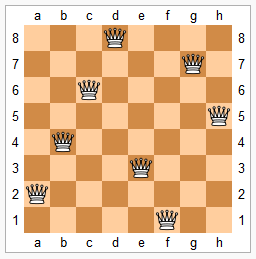
\includegraphics{8-queens.png}\\
\figcaption{Eight Queens}\label{fig:8-queens}
\end{center}

Given an integer $n$, return all distinct solutions to the n-queens puzzle.

Each solution contains a distinct board configuration of the n-queens' placement, where \fn{'Q'} and \fn{'.'} both indicate a queen and an empty space respectively.

For example,
There exist two distinct solutions to the 4-queens puzzle:
\begin{Code}
[
 [".Q..",  // Solution 1
  "...Q",
  "Q...",
  "..Q."],

 ["..Q.",  // Solution 2
  "Q...",
  "...Q",
  ".Q.."]
]
\end{Code}


\subsubsection{分析}
经典的深搜题。

\subsubsection{代码}
\begin{Code}
// LeetCode, N-Queens
// 深搜+剪枝
// 时间复杂度O(n!),空间复杂度O(n)
class Solution {
public:
    vector<vector<string> > solveNQueens(int n) {
        this->columns = vector<int>(n, 0);
        this->main_diag = vector<int>(2 * n, 0);
        this->anti_diag = vector<int>(2 * n, 0);

        vector<vector<string> > result;
        vector<int> C(n, 0);  // C[i]表示第i行皇后所在的列编号
        dfs(C, result, 0);
        return result;
    }
private:
    // 这三个变量用于剪枝
    vector<int> columns;  // 表示已经放置的皇后占据了哪些列
    vector<int> main_diag;  // 占据了哪些主对角线
    vector<int> anti_diag;  // 占据了哪些副对角线

    void dfs(vector<int> &C, vector<vector<string> > &result, int row) {
        const int N = C.size();
        if (row == N) { // 终止条件,也是收敛条件,意味着找到了一个可行解
            vector<string> solution;
            for (int i = 0; i < N; ++i) {
                string s(N, '.');
                for (int j = 0; j < N; ++j) {
                    if (j == C[i]) s[j] = 'Q';
                }
                solution.push_back(s);
            }
            result.push_back(solution);
            return;
        }

        for (int j = 0; j < N; ++j) {  // 扩展状态,一列一列的试
            const bool ok = columns[j] == 0 && main_diag[row + j] == 0 &&
                    anti_diag[row - j + N] == 0;
            if (!ok) continue;  // 剪枝:如果合法,继续递归
            // 执行扩展动作
            C[row] = j;
            columns[j] = main_diag[row + j] = anti_diag[row - j + N] = 1;
            dfs(C, result, row + 1);
            // 撤销动作
            // C[row] = 0;
            columns[j] = main_diag[row + j] = anti_diag[row - j + N] = 0;
        }
    }
};
\end{Code}


\subsubsection{相关题目}
\begindot
\item N-Queens II,见 \S \ref{sec:n-queens-ii}
\myenddot


\section{N-Queens II} %%%%%%%%%%%%%%%%%%%%%%%%%%%%%%
\label{sec:n-queens-ii}


\subsubsection{描述}
Follow up for N-Queens problem.

Now, instead outputting board configurations, return the total number of distinct solutions.


\subsubsection{分析}
只需要输出解的个数,不需要输出所有解,代码要比上一题简化很多。设一个全局计数器,每找到一个解就增1。


\subsubsection{代码}
\begin{Code}
// LeetCode, N-Queens II
// 深搜+剪枝
// 时间复杂度O(n!),空间复杂度O(n)
class Solution {
public:
    int totalNQueens(int n) {
        this->count = 0;
        this->columns = vector<int>(n, 0);
        this->main_diag = vector<int>(2 * n, 0);
        this->anti_diag = vector<int>(2 * n, 0);

        vector<int> C(n, 0);  // C[i]表示第i行皇后所在的列编号
        dfs(C, 0);
        return this->count;
    }
private:
    int count; // 解的个数
    // 这三个变量用于剪枝
    vector<int> columns;  // 表示已经放置的皇后占据了哪些列
    vector<int> main_diag;  // 占据了哪些主对角线
    vector<int> anti_diag;  // 占据了哪些副对角线

    void dfs(vector<int> &C, int row) {
        const int N = C.size();
        if (row == N) { // 终止条件,也是收敛条件,意味着找到了一个可行解
            ++this->count;
            return;
        }

        for (int j = 0; j < N; ++j) {  // 扩展状态,一列一列的试
            const bool ok = columns[j] == 0 &&
                    main_diag[row + j] == 0 &&
                    anti_diag[row - j + N] == 0;
            if (!ok) continue;  // 剪枝:如果合法,继续递归
            // 执行扩展动作
            C[row] = j;
            columns[j] = main_diag[row + j] =
                    anti_diag[row - j + N] = 1;
            dfs(C, row + 1);
            // 撤销动作
            // C[row] = 0;
            columns[j] = main_diag[row + j] =
                    anti_diag[row - j + N] = 0;
        }
    }
};
\end{Code}


\subsubsection{相关题目}
\begindot
\item N-Queens,见 \S \ref{sec:n-queens}
\myenddot


\section{Restore IP Addresses} %%%%%%%%%%%%%%%%%%%%%%%%%%%%%%
\label{sec:restore-ip-addresses}


\subsubsection{描述}
Given a string containing only digits, restore it by returning all possible valid IP address combinations.

For example:
Given \code{"25525511135"},

return \code{["255.255.11.135", "255.255.111.35"]}. (Order does not matter)


\subsubsection{分析}
必须要走到底部才能判断解是否合法,深搜。


\subsubsection{代码}
\begin{Code}
// LeetCode, Restore IP Addresses
// 时间复杂度O(n^4),空间复杂度O(n)
class Solution {
public:
    vector<string> restoreIpAddresses(string s) {
        vector<string> result;
        string ip; // 存放中间结果
        dfs(s, 0, 0, ip, result);
        return result;
    }

    /**
     * @brief 解析字符串
     * @param[in] s 字符串,输入数据
     * @param[in] startIndex 从s的哪里开始
     * @param[in] step 当前步骤编号,从0开始编号,取值为0,1,2,3,4表示结束了
     * @param[out] intermediate 当前解析出来的中间结果
     * @param[out] result 存放所有可能的IP地址
     * @return 无
     */
    void dfs(string s, size_t start, size_t step, string ip,
            vector<string> &result) {
        if (start == s.size() && step == 4) {  // 找到一个合法解
            ip.resize(ip.size() - 1);
            result.push_back(ip);
            return;
        }

        if (s.size() - start > (4 - step) * 3)
            return;  // 剪枝
        if (s.size() - start < (4 - step))
            return;  // 剪枝

        int num = 0;
        for (size_t i = start; i < start + 3; i++) {
            num = num * 10 + (s[i] - '0');

            if (num <= 255) {  // 当前结点合法,则继续往下递归
                ip += s[i];
                dfs(s, i + 1, step + 1, ip + '.', result);
            }
            if (num == 0) break;  // 不允许前缀0,但允许单个0
        }
    }
};
\end{Code}


\subsubsection{相关题目}
\begindot
\item 无
\myenddot


\section{Combination Sum} %%%%%%%%%%%%%%%%%%%%%%%%%%%%%%
\label{sec:combination-sum}


\subsubsection{描述}
Given a set of candidate numbers ($C$) and a target number ($T$), find all unique combinations in $C$ where the candidate numbers sums to $T$.

The same repeated number may be chosen from $C$ \emph{unlimited} number of times.

Note:
\begindot
\item All numbers (including target) will be positive integers.
\item Elements in a combination ($a_1, a_2, ..., a_k$) must be in non-descending order. (ie, $a_1 > a_2 > ... > a_k$).
\item The solution set must not contain duplicate combinations.
\myenddot

For example, given candidate set \fn{2,3,6,7} and target \fn{7}, 
A solution set is: 
\begin{Code}
[7] 
[2, 2, 3] 
\end{Code}


\subsubsection{分析}
无


\subsubsection{代码}
\begin{Code}
// LeetCode, Combination Sum
// 时间复杂度O(n!),空间复杂度O(n)
class Solution {
public:
    vector<vector<int> > combinationSum(vector<int> &nums, int target) {
        sort(nums.begin(), nums.end());
        vector<vector<int> > result; // 最终结果
        vector<int> intermediate; // 中间结果
        dfs(nums, target, 0, intermediate, result);
        return result;
    }

private:
    void dfs(vector<int>& nums, int gap, int start, vector<int>& intermediate,
            vector<vector<int> > &result) {
        if (gap == 0) {  // 找到一个合法解
            result.push_back(intermediate);
            return;
        }
        for (size_t i = start; i < nums.size(); i++) { // 扩展状态
            if (gap < nums[i]) return; // 剪枝

            intermediate.push_back(nums[i]); // 执行扩展动作
            dfs(nums, gap - nums[i], i, intermediate, result);
            intermediate.pop_back();  // 撤销动作
        }
    }
};
\end{Code}


\subsubsection{相关题目}
\begindot
\item Combination Sum II ,见 \S \ref{sec:combination-sum-ii}
\myenddot


\section{Combination Sum II} %%%%%%%%%%%%%%%%%%%%%%%%%%%%%%
\label{sec:combination-sum-ii}


\subsubsection{描述}
Given a set of candidate numbers ($C$) and a target number ($T$), find all unique combinations in $C$ where the candidate numbers sums to $T$.

The same repeated number may be chosen from $C$ \emph{once} number of times.

Note:
\begindot
\item All numbers (including target) will be positive integers.
\item Elements in a combination ($a_1, a_2, ..., a_k$) must be in non-descending order. (ie, $a_1 > a_2 > ... > a_k$).
\item The solution set must not contain duplicate combinations.
\myenddot

For example, given candidate set \fn{10,1,2,7,6,1,5} and target \fn{8}, 
A solution set is: 
\begin{Code}
[1, 7] 
[1, 2, 5] 
[2, 6] 
[1, 1, 6]
\end{Code}


\subsubsection{分析}
无


\subsubsection{代码}
\begin{Code}
// LeetCode, Combination Sum II
// 时间复杂度O(n!),空间复杂度O(n)
class Solution {
public:
    vector<vector<int> > combinationSum2(vector<int> &nums, int target) {
        sort(nums.begin(), nums.end()); // 跟第 50 行配合,
                                             // 确保每个元素最多只用一次
        vector<vector<int> > result;
        vector<int> intermediate;
        dfs(nums, target, 0, intermediate, result);
        return result;
    }
private:
    // 使用nums[start, nums.size())之间的元素,能找到的所有可行解
    static void dfs(vector<int> &nums, int gap, int start,
            vector<int> &intermediate, vector<vector<int> > &result) {
        if (gap == 0) {  //  找到一个合法解
            result.push_back(intermediate);
            return;
        }

        int previous = -1;
        for (size_t i = start; i < nums.size(); i++) {
            // 如果上一轮循环没有选nums[i],则本次循环就不能再选nums[i],
            // 确保nums[i]最多只用一次
            if (previous == nums[i]) continue;

            if (gap < nums[i]) return;  // 剪枝

            previous = nums[i];

            intermediate.push_back(nums[i]);
            dfs(nums, gap - nums[i], i + 1, intermediate, result);
            intermediate.pop_back();  // 恢复环境
        }
    }
};
\end{Code}


\subsubsection{相关题目}
\begindot
\item Combination Sum ,见 \S \ref{sec:combination-sum}
\myenddot


\section{Generate Parentheses } %%%%%%%%%%%%%%%%%%%%%%%%%%%%%%
\label{sec:generate-parentheses}


\subsubsection{描述}
Given $n$ pairs of parentheses, write a function to generate all combinations of well-formed parentheses.

For example, given $n = 3$, a solution set is:
\begin{Code}
"((()))", "(()())", "(())()", "()(())", "()()()"
\end{Code}

\subsubsection{分析}
小括号串是一个递归结构,跟单链表、二叉树等递归结构一样,首先想到用递归。

一步步构造字符串。当左括号出现次数$<n$时,就可以放置新的左括号。当右括号出现次数小于左括号出现次数时,就可以放置新的右括号。


\subsubsection{代码1}
\begin{Code}
// LeetCode, Generate Parentheses
// 时间复杂度O(TODO),空间复杂度O(n)
class Solution {
public:
    vector<string> generateParenthesis(int n) {
        vector<string> result;
        if (n > 0) generate(n, "", 0, 0, result);
        return result;
    }
    // l 表示 ( 出现的次数, r 表示 ) 出现的次数
    void generate(int n, string s, int l, int r, vector<string> &result) {
        if (l == n) {
            result.push_back(s.append(n - r, ')'));
            return;
        }
        generate(n, s + '(', l + 1, r, result);
        if (l > r) generate(n, s + ")", l, r + 1, result);
    }
};
\end{Code}


\subsubsection{代码2}
另一种递归写法,更加简洁。
\begin{Code}
// LeetCode, Generate Parentheses
// @author 连城 (http://weibo.com/lianchengzju)
class Solution {
public:
    vector<string> generateParenthesis (int n) {
        if (n == 0) return vector<string>(1, "");
        if (n == 1) return vector<string> (1, "()");
        vector<string> result;

        for (int i = 0; i < n; ++i)
            for (auto inner : generateParenthesis (i))
                for (auto outer : generateParenthesis (n - 1 - i))
                    result.push_back ("(" + inner + ")" + outer);

        return result;
    }
};
\end{Code}


\subsubsection{相关题目}
\begindot
\item Valid Parentheses, 见 \S \ref{sec:valid-parentheses}
\item Longest Valid Parentheses, 见 \S \ref{sec:longest-valid-parentheses}
\myenddot


\section{Sudoku Solver} %%%%%%%%%%%%%%%%%%%%%%%%%%%%%%
\label{sec:sudoku-solver}


\subsubsection{描述}
Write a program to solve a Sudoku puzzle by filling the empty cells.

Empty cells are indicated by the character \fn{'.'}.

You may assume that there will be only one unique solution.

\begin{center}
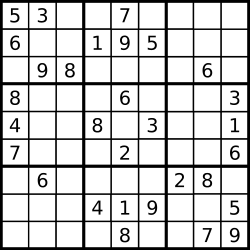
\includegraphics[width=150pt]{sudoku.png}\\
\figcaption{A sudoku puzzle...}\label{fig:sudoku}
\end{center}

\begin{center}
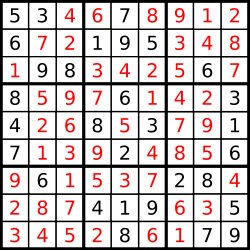
\includegraphics[width=150pt]{sudoku-solution.png}\\
\figcaption{...and its solution numbers marked in red}\label{fig:sudoku-solution}
\end{center}


\subsubsection{分析}
无。


\subsubsection{代码}
\begin{Code}
// LeetCode, Sudoku Solver
// 时间复杂度O(9^4),空间复杂度O(1)
class Solution {
public:
    bool solveSudoku(vector<vector<char> > &board) {
        for (int i = 0; i < 9; ++i)
            for (int j = 0; j < 9; ++j) {
                if (board[i][j] == '.') {
                    for (int k = 0; k < 9; ++k) {
                        board[i][j] = '1' + k;
                        if (isValid(board, i, j) && solveSudoku(board))
                            return true;
                        board[i][j] = '.';
                    }
                    return false;
                }
            }
        return true;
    }
private:
    // 检查 (x, y) 是否合法
    bool isValid(const vector<vector<char> > &board, int x, int y) {
        int i, j;
        for (i = 0; i < 9; i++) // 检查 y 列
            if (i != x && board[i][y] == board[x][y])
                return false;
        for (j = 0; j < 9; j++) // 检查 x 行
            if (j != y && board[x][j] == board[x][y])
                return false;
        for (i = 3 * (x / 3); i < 3 * (x / 3 + 1); i++)
            for (j = 3 * (y / 3); j < 3 * (y / 3 + 1); j++)
                if (i != x && j != y && board[i][j] == board[x][y])
                    return false;
        return true;
    }
};
\end{Code}


\subsubsection{相关题目}
\begindot
\item Valid Sudoku, 见 \S \ref{sec:valid-sudoku}
\myenddot


\section{Word Search} %%%%%%%%%%%%%%%%%%%%%%%%%%%%%%
\label{sec:word-search}


\subsubsection{描述}
Given a 2D board and a word, find if the word exists in the grid.

The word can be constructed from letters of sequentially adjacent cell, where \fn{"adjacent"} cells are those horizontally or vertically neighbouring. The same letter cell may not be used more than once.

For example,
Given board =
\begin{Code}
[
  ["ABCE"],
  ["SFCS"],
  ["ADEE"]
]
\end{Code}
word = \fn{"ABCCED"}, -> returns \fn{true},\\
word = \fn{"SEE"}, -> returns \fn{true},\\
word = \fn{"ABCB"}, -> returns \fn{false}.


\subsubsection{分析}
无。


\subsubsection{代码}
\begin{Code}
// LeetCode, Word Search
// 深搜,递归
// 时间复杂度O(n^2*m^2),空间复杂度O(n^2)
class Solution {
public:
    bool exist(vector<vector<char> > &board, string word) {
        const int m = board.size();
        const int n = board[0].size();
        vector<vector<bool> > visited(m, vector<bool>(n, false));
        for (int i = 0; i < m; ++i)
            for (int j = 0; j < n; ++j)
                if (dfs(board, word, 0, i, j, visited))
                    return true;
        return false;
    }
private:
    static bool dfs(const vector<vector<char> > &board, const string &word,
            int index, int x, int y, vector<vector<bool> > &visited) {
        if (index == word.size())
            return true; // 收敛条件

        if (x < 0 || y < 0 || x >= board.size() || y >= board[0].size())
            return false;  // 越界,终止条件

        if (visited[x][y]) return false; // 已经访问过,剪枝

        if (board[x][y] != word[index]) return false; // 不相等,剪枝

        visited[x][y] = true;
        bool ret = dfs(board, word, index + 1, x - 1, y, visited) || // 上
                dfs(board, word, index + 1, x + 1, y, visited)    || // 下
                dfs(board, word, index + 1, x, y - 1, visited)    || // 左
                dfs(board, word, index + 1, x, y + 1, visited);      // 右
        visited[x][y] = false;
        return ret;
    }
};
\end{Code}


\subsubsection{相关题目}
\begindot
\item 无
\myenddot


\section{小结} %%%%%%%%%%%%%%%%%%%%%%%%%%%%%%
\label{sec:dfs-template}


\subsection{适用场景}

\textbf{输入数据}:如果是递归数据结构,如单链表,二叉树,集合,则百分之百可以用深搜;如果是非递归数据结构,如一维数组,二维数组,字符串,图,则概率小一些。

\textbf{状态转换图}:树或者图。

\textbf{求解目标}:必须要走到最深(例如对于树,必须要走到叶子节点)才能得到一个解,这种情况适合用深搜。


\subsection{思考的步骤}
\begin{enumerate}
\item 是求路径条数,还是路径本身(或动作序列)?深搜最常见的三个问题,求可行解的总数,求一个可行解,求所有可行解。
    \begin{enumerate}
	\item 如果是路径条数,则不需要存储路径。
    \item 如果是求路径本身,则要用一个数组\fn{path[]}存储路径。跟宽搜不同,宽搜虽然最终求的也是一条路径,但是需要存储扩展过程中的所有路径,在没找到答案之前所有路径都不能放弃;而深搜,在搜索过程中始终只有一条路径,因此用一个数组就足够了。
    \end{enumerate}

\item 只要求一个解,还是要求所有解?如果只要求一个解,那找到一个就可以返回;如果要求所有解,找到了一个后,还要继续扩展,直到遍历完。广搜一般只要求一个解,因而不需要考虑这个问题(广搜当然也可以求所有解,这时需要扩展到所有叶子节点,相当于在内存中存储整个状态转换图,非常占内存,因此广搜不适合解这类问题)。

\item 如何表示状态?即一个状态需要存储哪些些必要的数据,才能够完整提供如何扩展到下一步状态的所有信息。跟广搜不同,深搜的惯用写法,不是把数据记录在状态\fn{struct}里,而是添加函数参数(有时为了节省递归堆栈,用全局变量),\fn{struct}里的字段与函数参数一一对应。

\item 如何扩展状态?这一步跟上一步相关。状态里记录的数据不同,扩展方法就不同。对于固定不变的数据结构(一般题目直接给出,作为输入数据),如二叉树,图等,扩展方法很简单,直接往下一层走,对于隐式图,要先在第1步里想清楚状态所带的数据,想清楚了这点,那如何扩展就很简单了。

\item 关于判重
    \begin{enumerate}
    \item 是否需要判重?如果状态转换图是一棵树,则不需要判重,因为在遍历过程中不可能重复;如果状态转换图是一个DAG,则需要判重。这一点跟BFS不一样,BFS的状态转换图总是DAG,必须要判重。
    \item 怎样判重?跟广搜相同,见第 \S \ref{sec:bfs-template} 节。同时,DAG说明存在重叠子问题,此时可以用缓存加速,见第8步。
    \end{enumerate}

\item 终止条件是什么?终止条件是指到了不能扩展的末端节点。对于树,是叶子节点,对于图或隐式图,是出度为0的节点。

\item {收敛条件是什么?收敛条件是指找到了一个合法解的时刻。如果是正向深搜(父状态处理完了才进行递归,即父状态不依赖子状态,递归语句一定是在最后,尾递归),则是指是否达到目标状态;如果是逆向深搜(处理父状态时需要先知道子状态的结果,此时递归语句不在最后),则是指是否到达初始状态。

由于很多时候终止条件和收敛条件是是合二为一的,因此很多人不区分这两种条件。仔细区分这两种条件,还是很有必要的。

为了判断是否到了收敛条件,要在函数接口里用一个参数记录当前的位置(或距离目标还有多远)。如果是求一个解,直接返回这个解;如果是求所有解,要在这里收集解,即把第一步中表示路径的数组\fn{path[]}复制到解集合里。}

\item 如何加速?
    \begin{enumerate}
    \item 剪枝。深搜一定要好好考虑怎么剪枝,成本小收益大,加几行代码,就能大大加速。这里没有通用方法,只能具体问题具体分析,要充分观察,充分利用各种信息来剪枝,在中间节点提前返回。
    \item 缓存。
        \begin{enumerate}
            \item 前提条件:状态转换图是一个DAG。DAG=>存在重叠子问题=>子问题的解会被重复利用,用缓存自然会有加速效果。如果依赖关系是树状的(例如树,单链表等),没必要加缓存,因为子问题只会一层层往下,用一次就再也不会用到,加了缓存也没什么加速效果。
            \item 具体实现:可以用数组或HashMap。维度简单的,用数组;维度复杂的,用HashMap,C++有\fn{map},C++ 11以后有\fn{unordered_map},比\fn{map}快。
        \end{enumerate}
    
    \end{enumerate}
\end{enumerate}

拿到一个题目,当感觉它适合用深搜解决时,在心里面把上面8个问题默默回答一遍,代码基本上就能写出来了。对于树,不需要回答第5和第8个问题。如果读者对上面的经验总结看不懂或感觉“不实用”,很正常,因为这些经验总结是我做了很多题目后总结出来的,从思维的发展过程看,“经验总结”要晚于感性认识,所以这时候建议读者先做做前面的题目,积累一定的感性认识后,再回过头来看这一节的总结,一定会有共鸣。


\subsection{代码模板}

\begin{Codex}[label=dfs_template.cpp]
/**
 * dfs模板.
 * @param[in] input 输入数据指针
 * @param[out] path 当前路径,也是中间结果
 * @param[out] result 存放最终结果
 * @param[inout] cur or gap 标记当前位置或距离目标的距离
 * @return 路径长度,如果是求路径本身,则不需要返回长度
 */
void dfs(type &input, type &path, type &result, int cur or gap) {
    if (数据非法) return 0;   // 终止条件
    if (cur == input.size()) { // 收敛条件
    // if (gap == 0) {
        将path放入result
    }

    if (可以剪枝) return;

    for(...) { // 执行所有可能的扩展动作
        执行动作,修改path
        dfs(input, step + 1 or gap--, result);
        恢复path
    }
}
\end{Codex}


\subsection{深搜与回溯法的区别}
深搜(Depth-first search, DFS)的定义见\myurl{http://en.wikipedia.org/wiki/Depth_first_search},回溯法(backtracking)的定义见\myurl{http://en.wikipedia.org/wiki/Backtracking}

\textbf{回溯法 = 深搜 + 剪枝}。一般大家用深搜时,或多或少会剪枝,因此深搜与回溯法没有什么不同,可以在它们之间画上一个等号。本书同时使用深搜和回溯法两个术语,但读者可以认为二者等价。

深搜一般用递归(recursion)来实现,这样比较简洁。

深搜能够在候选答案生成到一半时,就进行判断,抛弃不满足要求的答案,所以深搜比暴力搜索法要快。


\subsection{深搜与递归的区别}
\label{sec:dfs-vs-recursion}

深搜经常用递归(recursion)来实现,二者常常同时出现,导致很多人误以为他俩是一个东西。

深搜,是逻辑意义上的算法,递归,是一种物理意义上的实现,它和迭代(iteration)是对应的。深搜,可以用递归来实现,也可以用栈来实现;而递归,一般总是用来实现深搜。可以说,\textbf{递归一定是深搜,深搜不一定用递归}。

递归有两种加速策略,一种是\textbf{剪枝(prunning)},对中间结果进行判断,提前返回;一种是\textbf{缓存},缓存中间结果,防止重复计算,用空间换时间。

其实,递归+缓存,就是 memorization。所谓\textbf{memorization}(翻译为备忘录法,见第 \S \ref{sec:dp-vs-memorization}节),就是"top-down with cache"(自顶向下+缓存),它是Donald Michie 在1968年创造的术语,表示一种优化技术,在top-down 形式的程序中,使用缓存来避免重复计算,从而达到加速的目的。

\textbf{memorization 不一定用递归},就像深搜不一定用递归一样,可以在迭代(iterative)中使用 memorization 。\textbf{递归也不一定用 memorization},可以用memorization来加速,但不是必须的。只有当递归使用了缓存,它才是 memorization 。

既然递归一定是深搜,为什么很多书籍都同时使用这两个术语呢?在递归味道更浓的地方,一般用递归这个术语,在深搜更浓的场景下,用深搜这个术语,读者心里要弄清楚他俩大部分时候是一回事。在单链表、二叉树等递归数据结构上,递归的味道更浓,这时用递归这个术语;在图、隐式图等数据结构上,深搜的味道更浓,这时用深搜这个术语。
